% This file is iccc.tex.  It contains the formatting instructions for and acts as a template for submissions to ICCC.  It borrows liberally from the AAAI and IJCAI formats and instructions.  It uses the files iccc.sty, iccc.bst and iccc.bib, the first two of which also borrow liberally from the same sources.

\documentclass[letterpaper]{article}
\usepackage{iccc}

\usepackage{graphicx}
\usepackage{times}
\usepackage{helvet}
\usepackage{courier}
\pdfinfo{
	/Title (Anything2vec: generalizing word2vec via the use of meaningful contexts)
	/Subject (Proceedings of ICCC)
	/Author (ICCC)}
% The file iccc.sty is the style file for ICCC proceedings.
%

%\title{Anything2vec: generalizing word2vec via the use of meaningful
%	contexts}
% Add something about its application to trope description - JJ 
%\author{Dan Ventura\\
%Computer Science Department\\
%Brigham Young University\\
%Provo, UT 84602  USA\\
%ventura@cs.byu.edu\\
%}
\setcounter{secnumdepth}{0}

\begin{document} 
	% \maketitle
	\begin{abstract}
		\begin{quote}
			% From the old paper:
			%   Word2vec has been a very successful algorithm that is able to give a
			% semantic representation to words on a corpus based in the context
			% they appear. In this paper we will try to extend this concept to
			% other {\em unordered} contexts. We will try to define this context
			% for movie (and TV) tropes.
			In this paper we present a generalized approach to extend the use of word2vec for non-traditional NLP (Natural Language Processing). In order to exemplify the idea, we use tvtropes dataset (trope names and film names only) to create a text corpus in order to give contextual information to any piece of data.
		\end{quote}
	\end{abstract}
	
	% From the old paper:
	% What are tropes and why we are interested
	
	% We need to find an embedding for tropes that allows us to do trope arithmetic and also process them, and movies in which they are used, in an uniform way.
	
	% We propose trope2vec
	
	% We analyse how it allows to explore the trope space and find
	% similarities between them.
	
	\section{Introduction}
	
	% Motivation: we need to have a representation that is
	% * That includes the context of the trope
	% * relatively compact
	% * capable of doing arithmetic
	% * uniform for tropes and movies.
	
	This work aims to find a knowledge representation and a new
	methodology to apply machine learning techniques to entities without a
	natural language context. % ← You go from objectives
	% To what you will be doing →
	To exemplify this new methodology, tropes and films from tvtropes.org
	are used. That representation and methodology will let us, for
	example, to discover which set of tropes will be affordable to create a
	new block buster film or a new best seller book.
	
	% Before telling what you are going to be doing, you need to show the
	% context and the motivation in one or two paragraphs - JJ
	
	% And here you say *how* you will be doing it. Still too soon. This
	% should go to the methodology, not the introduction. You are going to
	% create embedding  for tropes, and you say why. Later, in the
	% methodology, you say how you will be obtaining those tropes - JJ
	Tv Tropes (tvtropes.org) is a collaborative website created in 2004 to
	share information about tips, narrative or cinematographic techniques
	used in creative works such as movies, tv series, advertising,
	videogames, sports, comics or books; latest iterations even include
	{\em real life} tropes.
	% This is a definition of tropes, which is context, not
	% methodology. Move it up. Also use proper referencing, and cite other
	% sources - JJ
	Tvtropes.org defines tropes as:
	"a storytelling device or convention, a shortcut for describing
	situations the storyteller can reasonably assume the audience will
	recognize." Articles to describe tropes are written usually with a very
	expressive and non-formal vocabulary. Each film, TV series or other
	fiction element usually includes a description and a list of associated
	tropes. Tropes pages usually contains a description followed by a list
	of films or a narrative resource that uses this trope.
	
	% This is what you want to do to achieve the objectives. It belongs in
	% the introduction, but with a certain level of brevity. It's also
	% motivation for the paper - JJ
	To represent tropes, we decided to use embedding vectors for each
	trope. This representation should allow us to perform concept
	arithmetic. This property will be very interesting since our goal is
	to determine, for example, which group of tropes must have a
	successful film. Applying arithmetic of concepts about tropes we
	could, for example, find classic western movies, which have their main
	narrative characteristics, but the western one is replaced by space
	adventure trope. in order to obtain the set of embedding vectors
	associated with the tropes we will use word2vec
	\cite{mikolov2013}. Since the development of this technique in 2013
	word2vec is one of the techniques for the generation of embedding
	vectors from natural language (NLP) most used. However, word2vec has
	not only been used to obtain embedding vectors of texts in natural
	language. Other works like \cite{kazama2018} have shown that it is
	possible to use word2vec to obtain vectors from non-NLP information
	sources. Our approach is based on the use of the fundamental elements
	of information (in our case the tropes) to generate an artificial
	narrative or corpus that can give a similar meaning to the concepts
	that they would have in a text written by humans. This artificially
	created text should represent the relationships between entities in
	the same way that a human would relate them in a descriptive text
	about these entities. If the artificial corpus is correctly
	constructed, it should produce some embedding vectors with the
	capacity to offer us a correct arithmetic of concepts. 
	
	% How we want to solve that problem: we think that an adaptation of word2vec should be possible
	% This is what you say above - JJ
	
	% One of the most important elements in NLP (Natural Language Processing) is the context where words appear inside a text. One of the most popular algorithms to associate numerical vectors to words is word2vec \cite{mikolov2013}. This algorithm use words that are before and after a target word in order to contextualize words. But, what happens if we don't have a text to start analysing words? What happens if we only have relationships between terms like this trope appear in this film? For this type of problem, we purpose a generalization in the use of word2vec algorithm that let to build a context for related terms. 
	
	% How we do it:
	% * Methodology for creating the context of every trope
	% * Methodology for representing movies using trope vector
	% * How we evaluate the goodness of the set of movies/tropes chosen.
	
	% Our results
	% * Clustering
	% * Graph representation
	% * Movie representation
	% * Example of synthetic movie generation.
	
	The rest of the paper is organized as follows. Next we present the
	state of the art in using embedding for problems other than language
	processing, as well as an overview of the use of tropes for narrative
	generation. The methodology is presented next in Section
	\ref{sec:met}, with results presented in Section \ref{sec:res}
	followed by the conclusion that closes the paper.
	
	
	\section{State of the art}
	
	Unlike systems such as MovieLens \cite{10.1145/2827872}, which focus
	on recommendation, our ultimate
	interest in representing movie tropes lies in the possibility of
	generating narratives \cite{10.5555/931357} that are optimal from some point of view (mainly
	coherence) from a set of tropes. Out of all the possible methods to
	generate narratives \cite{van2019narrative} this is one that has
	probably been explored the least; Sullivan et
	al. \cite{10.1145/3235765.3235819} used tropes in the tarot deck to
	generate narratives via combinations, but other than that, in general
	the presence of tropes has been used more for evaluation of generated
	narratives \cite{gervas2012story} that as part of the generation
	itself; in general, tropes are understood as constraints for
	characters or plots \cite{Thompson18NarrativeEvents}, but, of course,
	there are many kind of tropes and some of them can be converted
	directly into plots; for instance, {\sf AgeStereotypicalFood} informs
	of the fact that eating or talking about food will be introduced into
	the narrative.
	
	This work has been inspired by other that have used
	word2vec-like embeddings for purposes that are totally
	unrelated to natural language; a good survey is presented in
	\cite{nonnlp19}. In general, creating embeddings out of data
	is done with several purposes: reducing dimensionality, but
	also trying to create a data representation with semantics; as
	a side effect, this data representation will enable ``content
	arithmetics''. In our previous work
	\cite{doi:10.1111/exsy.12525} we used a direct representation
	of tropes; every dimension in a vector represented a trope,
	once less frequent ones had been excluded. However, this left
	out many possibly meaningful tropes, and still the size of the
	vectors was huge, representing its own challenge when using
	them in a deep learning algorithm.
	
	This was one of the intentions of Kazama et al. in
	\cite{kazama2018}, which is actually the paper that inspired
	our work. The content they wanted to represent was the concept
	of ``regional cuisine'', so that a regional cuisine embedding
	could be added or substracted from the embedding of a dish to
	create a new, equivalent one in that new regional
	environment. The kind of data they were working with is
	similar to the one we use in this paper: dish ingredients. As
	in our case, there's no natural order in the ingredients, but
	unlike our case, the amount of ingredients that are used in a
	dish are really limited, at least if you exclude
	seasoning. But they achieved their objective: being able to do
	recipe arithmetics, but also create meaningful maps of food
	that can be used in deep learning or any other environment.
	
	Most other applications are similar, in a way, to this one,
	and most of them are also recent. There was a publication in
	the Twitter engineering blog \cite{twitter:embeddings},
	apparently pointing to their use studying the social networks
	of users. Initial work was done by Grbovic et al. applied it to product recommendation
	\cite{Grbovic2015}, Vasile et al. applied it to product
	recommendation systems \cite{vasile2016} while McAuley et
	al. \cite{DBLP:journals/corr/McAuleyPL15} used embedding
	arithmetics to find complementary products to others that had
	been already purchased; these articles were
	probably ones of the first to use this kind of
	representation.
	
	Word embeddings to create clustering, however, go back at
	least to Kohonen's work in the 90s
	\cite{kohonen1997exploration}, which tried to create
	embeddings by assigning a word a vector created from averaging
	randomly created vectors initially assigned to its neighboring
	vectors. This work was extended to ant clustering algorithms
	to create word clusterings by Ramos et
	al. \cite{DBLP:journals/corr/abs-cs-0412075}.
	
	The fact that the variety of data embeddings have been applied
	to, as well as the kind of applications created with is so
	wide, has encouraged us to apply it to the study of movies via
	their tropes, as well as its eventual optimization.
	
	\section{Methodology}
	\label{sec:met}
	
	1. Download TvTropes dataset \\
	2. Select films with number of tropes less than a certain number of tropes. The idea is to create a corpus with sentences constructed by permutations of sub-sets of tropes. \\
	3. Build the corpus with permutations of tropes in each film \\
	
	To represent tropes we decided to use embedding vectors for
	each trope. This representation should allow us to perform
	concept arithmetic. This property will be very interesting
	since our goal is to determine, for example, which group of
	tropes must have a successful film. Applying arithmetic of
	concepts about tropes we could, for example, find classic
	western movies, which have their main narrative
	characteristics, but the western one is replaced by space
	adventure trope. in order to obtain the set of embedding vectors
	associated with the tropes we will use word2vec
	\cite{mikolov2013}. Since the development of this technique in
	2013 word2vec is one of the techniques for the generation of
	embedding vectors from natural language (NLP) most
	used. However, word2vec has not only been used to obtain
	embedding vectors of texts in natural language. Other works
	like \cite{kazama2018} have shown that it is possible to use
	word2vec to obtain vectors from non-NLP information
	sources. Our approach is based on the use of the fundamental
	elements of information (in our case the tropes) to generate
	an artificial narrative or corpus that can give a similar
	meaning to the concepts that they would have in a text written
	by humans. This artificially created text should represent the
	relationships between entities in the same way that a human
	would relate them in a descriptive text about these
	entities. If the artificial corpus is correctly constructed,
	it should produce some embedding vectors with the capacity to
	offer us a correct arithmetic of concepts.
	
	To obtain this artificial corpus, we place together entities
	that are connected. In the example of tvtropes, we will
	generate the artificial corpus generating phrases that put
	together film tropes. In order to generate the corpus, we will
	select films that have a maximum of 15 tropes. We take this
	initial limit since we will generate all the variations
	without repetitions of 15 elements taken in groups of n
	elements. his method can give us enough size corpus to train
	the model using word2vec algorithm.
	In order to generate the artificial corpus, we have followed this procedure. We have selected those films that have a maximum of MAX\_TROPES tropes and eliminating those that have zero or 1 trope.  

\begin{table}[t]
	\centering
	\begin{tabular}{|p{0.20\linewidth}|p{0.2\linewidth}|p{0.2\linewidth}|p{0.2\linewidth}|}
		\hline
		\textbf{(MaxTrop, NgramSize)}& \textbf{(16,9)} & \textbf{(15, 9)} & \textbf{(12,7)}\\
		\hline
		\hline
		Tropes Subset Size&8125&7383& 5500\\
		\hline
		Film Subset Size&2686&2380& 1674\\
		\hline
		Corpus File Size (MB)&747&264& 32\\
		\hline
	    Word2vec Model file Size(MB)&5.6&4.9&4.9\\
		\hline
		Vocab Size& 7078 & 6173 & 4653\\
		\hline
		Words in train file& 48893099 &17386514&2056372\\
		\hline
		Time real&179m53.655s&61m8.348s&6m49.522s\\
        \hline
		Time user&524m50.420s&177m48.830s&19m53.780s\\
		\hline
	    Time sys&8m51.080s&3m10.870s&0m19.780s\\
		\hline
		
	\end{tabular}
	\caption{Characteristics of different corpus sizes and word2vec models created by varying MAX\_TROPES and NGRAM\_SIZE (word2vec argument min-count = 5). Execution time for i7 5500u 2.40 Ghz 16GB RAM}
	\label{tab:corpusSize}
\end{table}
	
	
	
	This filtering process generates a reduced set of tropes. Table \ref{tab:corpusSize} shows characteristics of different sets of films, tropes and generated corpus. Full set of tropes have 25405 different tropes. Figure \ref{fig:tropesdistributionasociatedtofilms} shows the accumulative distribution of tropes and films, where 250 threshold will include more than 25000 tropes. 
	
	
	In case of subset of films with number of tropes between 15 and 2 tropes has only 6524 different tropes. 
    It is important to check if our subset of tropes is relevant within the total set of tropes. To do so, we order the tropes by number of times it appears in a movie. In case of subset of tropes from films between 15 and 2 tropes, our subset cover the 99,2 percent of the 250 most popular tropes, so we can consider it a representative subset. 
	
	
	Tvtropes dataset has 673258 pairs film-trope. 73917 duplicate values in pairs. After apply word2vect to artificially created corpus, a set of embedding vectors will be created. The embedding vector integrate information about the context of a certain word and it is easy to find the relationships with other terms in corpus.\\
	To obtain this artificial corpus, we place together entities that are connected. In the example of tvtropes, we create the artificial corpus generating phrases that put together tropes used in a film. In order to generate the corpus, we will select films that have MAX\_TROPES tropes. We take this initial limit since we will generate all the variations without repetitions of MAX\_TROPES elements taken in groups of NGRAM\_SIZE elements. This method can give us a corpus with hundred of Mega Bytes to train the model using word2vec algorithm. \\
	
	\begin{figure}
		\centering
		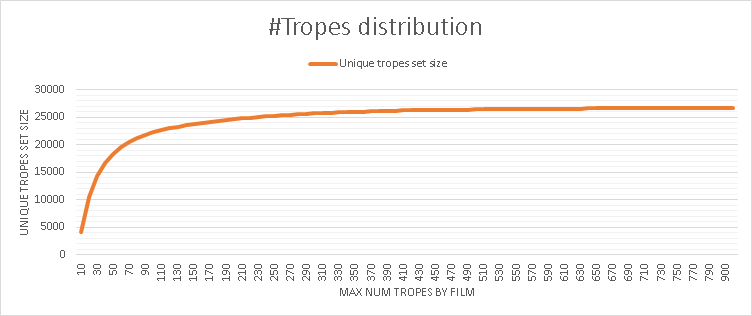
\includegraphics[width=1\linewidth]{../images/tropes_distribution_chart.png}
		\caption{Accumulative distribution of tropes associated to films}
		\label{fig:tropesdistributionasociatedtofilms}
	\end{figure}
	
	The challenge now is how to create a corpus that will be useful to find relationships between tropes and films. Each film has a description and a list of tropes, and each trope have a description and a list of films that uses this trope. Initially our dataset obtained from tvtropes.org 13th December 2019 included 12360 films and 26742 different tropes (25405 after remove duplicates). The film with higher number of tropes has 1028 tropes and the film with minimum number of tropes has 0 tropes. Tvtropes dataset has 673258 pairs film-trope. 73917 duplicate values in pairs. After apply word2vect to artificially created corpus, a set of embedding vectors will be created. The embedding vector integrate information about the context of a certain word and it is easy to find the relationships with other terms in corpus.\\
	
	The size of the corpus of variations without repetition of 15 tropes taken from 9 in 9 is 288 Mbytes. 9-size phrases have been created by making variations without repetition and ordering the result randomly \\
	
	\begin{center}
		
		${v}_{m,n} = m.(m-1).(m-2)...(m-n+1)$
		${v}_{15,9} = 1816214400$
		
	\end{center}
	
	Below first lines of corpus generated file:\\
	\texttt{    
		hiredguns annoyingarrows naughtynuns attemptedrape nonindicativename badhabits characterdevelopment automatonhorses cigarfuselighting    cigarfuselighting hiredguns badhabits annoyingarrows nuntooholy characterdevelopment naughtynuns automatonhorses attemptedrape    onlyinitforthemoney attemptedrape cigarfuselighting badhabits annoyingarrows characterdevelopment automatonhorses }\\
	
	%       % This kind of thing does not belong in a paper 
	%     Following line represent word2vec train parameters:\\
	% \begin{verbatim}
	% /word2vec 
	% -train ngrams_15_taken_9.txt 
	% -output ngrams_15_taken_9.bin 
	% -cbow 1 -size 200 -window 8 
	% -negative 25 -hs 0 
	% -sample 1e-4 -threads 20 
	% -binary 1 -iter 15
	% \end{verbatim}
	
	% There's no need to say what to do; focus on the results and the
	% methodology. Mechanical steps can be explained in the repository.
	
	
	4. Build word2vec model. After that we will have a numerical vector for each trope. \\
	   
	   Once we have obtained the file with the corpus for training, using the word2vec package https://github.com/tmikolov/word2vec created by
	   \cite{mikolov2013} we run word2vec program to obtain trained model. This model will help us to obtain a embedding vector associated to each trope.
	   In our case, the corpus does not contain stop-words and other words lacking information. For this reason we have performed different tests with
	   word2vec by modifying the MIN\_COUNT parameter that eliminates words that appear less than MIN\_COUNT times. Table \ref{tab:variations-with-min-count-argument-15-9}
	   shows different details of the model and its creation process by varying the argument mentioned above.
	   We have detected that the same trope can be written in different ways. The way to separate the words that appear in the name of the trope is to write
	    the first letter in uppercase. We have found that sometimes for the same trope the sequence of cartoons in upper and lower case is not the same. 
	   In order to prevent the same trope from being taken as a different word, we have made a filter to convert troop names to lowercase.
	   
	   
	\begin{table}[t]
		\centering
		\begin{tabular}{|p{0.20\linewidth}|p{0.2\linewidth}|p{0.2\linewidth}|p{0.2\linewidth}|}
			\hline
			\textbf{(MaxTrop, NgramSize, Min Count)}& \textbf{(15, 9, 1)} & \textbf{(15,9, 3)} & \textbf{(15, 9, 5)}\\
			\hline
			\hline
			Vocab Size& 7384 & 6197 & 6173 \\
			\hline
			Words in train file& 17387907 & 17386591 & 17386514 \\
			\hline
			Time real&58m36.227s&57m25.768s&61m8.348s\\
			\hline
			Time user&170m48.400s&167m25.700s&177m48.830s\\
			\hline
			Time sys&2m45.900s&2m38.900s&3m10.870s\\
			\hline
			
		\end{tabular}
		\caption{Characteristics of different word2vec models created by varying the MIN\_COUNT argument. Execution time for i7 5500u 2.40 Ghz 16GB RAM}
		\label{tab:variations-with-min-count-argument-15-9}
	\end{table}	
	
	
	5. Visualize tropes vector space in order to detect clusters and possible data organization. \\
	   In order to verify that the model built with word2vec fulfills its purpose, we need to perform different checks. On the one hand, 
	   we must verify that the relations established between tropes of the model correspond to reality. 
	   Visualizing relationships between tropes in generated model can help us to verify the goodness of the model.
	   Therefore, the next task will be to generate a file with the numerical vector associated with each trope. 
	   To generate this file we have used a script that uses Gensim, an Open Source python library that include functions to manipulate
	   word2vec bin files.
	   Table \ref{tab:200dims-vectors-associated-to-tropes} shows the results in the number of tropes associated with vectors depending 
	   on the MIN\_COUNT parameter (1, 3 or 5). We can observe that for the value of MIN\_COUNT = 1 we obtain a vector associated with each trope, 
	   however for values of MIN\_COUNT 3 or 5 the vectors obtained are reduced. 
	   	\begin{table}[t]
	   	\centering
	   	\begin{tabular}{|p{0.20\linewidth}|p{0.2\linewidth}|p{0.2\linewidth}|p{0.2\linewidth}|}
	   		\hline
	   		\textbf{(MaxTrop, NgramSize, Min Count)}& \textbf{(15, 9, 1)} & \textbf{(15,9, 3)} & \textbf{(15, 9, 5)}\\
	   		\hline
	   		\hline
	   		Tropes with vector&7383  & 6196 & 6172 \\
	   		\hline
	   		Tropes without vector& 0 & 1187 & 1211 \\
	   		\hline
	   		Total tropes&7383&7383&7383\\
	   		\hline
	   		
	   	\end{tabular}
	   	\caption{200 dims vectors associated to tropes}
	   	\label{tab:200dims-vectors-associated-to-tropes}
	   \end{table}	
	   
	6. Create a Vector for each film as the sumatory of all tropes vectors. \\
	
	\section{Results}
	\label{sec:res}
	
	\section{Conclusions, discussion and future work}
	
	\section{Acknowledgments}
	
	\bibliographystyle{iccc}
	\bibliography{iccc}
	
\end{document}
